\section{计算法}
\subsection{面积法}
\begin{proposition}
    对任意 $\triangle ABC$,设$BC=a,AC=b,AB=c$。其面积可以表示为
    $$S_{\triangle ABC} =\frac{1}{2}bc\sin A=\frac{1}{2}ac\sin B=\frac{1}{2}ab\sin C$$
\end{proposition}
\begin{proof}
    过点A作BC的垂线交BC于D点,由三角形面积公式可知
    $$S_{\triangle ABC} = \frac{1}{2} BC \cdot AD = \frac{1}{2} a \cdot (\sin B \cdot AB) = \frac{1}{2} ac \sin B.$$
    其他同理可以证明。
\end{proof}


\subsection{三角法}
\begin{proposition}
    给定$0<\alpha_1,\alpha_2,\beta_1,\beta_2<180^\circ$,满足$\alpha_1+\beta_1=\alpha_2+\beta_2 < 180^\circ$,若
    $$
    \frac{\sin\alpha_1}{\sin\beta_1}= \frac{\sin\alpha_2}{\sin\beta_2},
    $$
    则一定有$\alpha_1=\alpha_2,\quad \beta_1 =\beta_2$。
\end{proposition}


\newpage 
\subsection{分角线定理}
\begin{theorem}[分角线定理]
    在$\triangle ABC$中,D是BC所在直线上异于B、C的一点,连结AD,则有
    $$
    \frac{BD}{DC} = \frac{AB\sin \angle BAD}{AC \sin \angle CAD}.
    $$
\end{theorem}
\begin{figure}[ht]
    \centering
    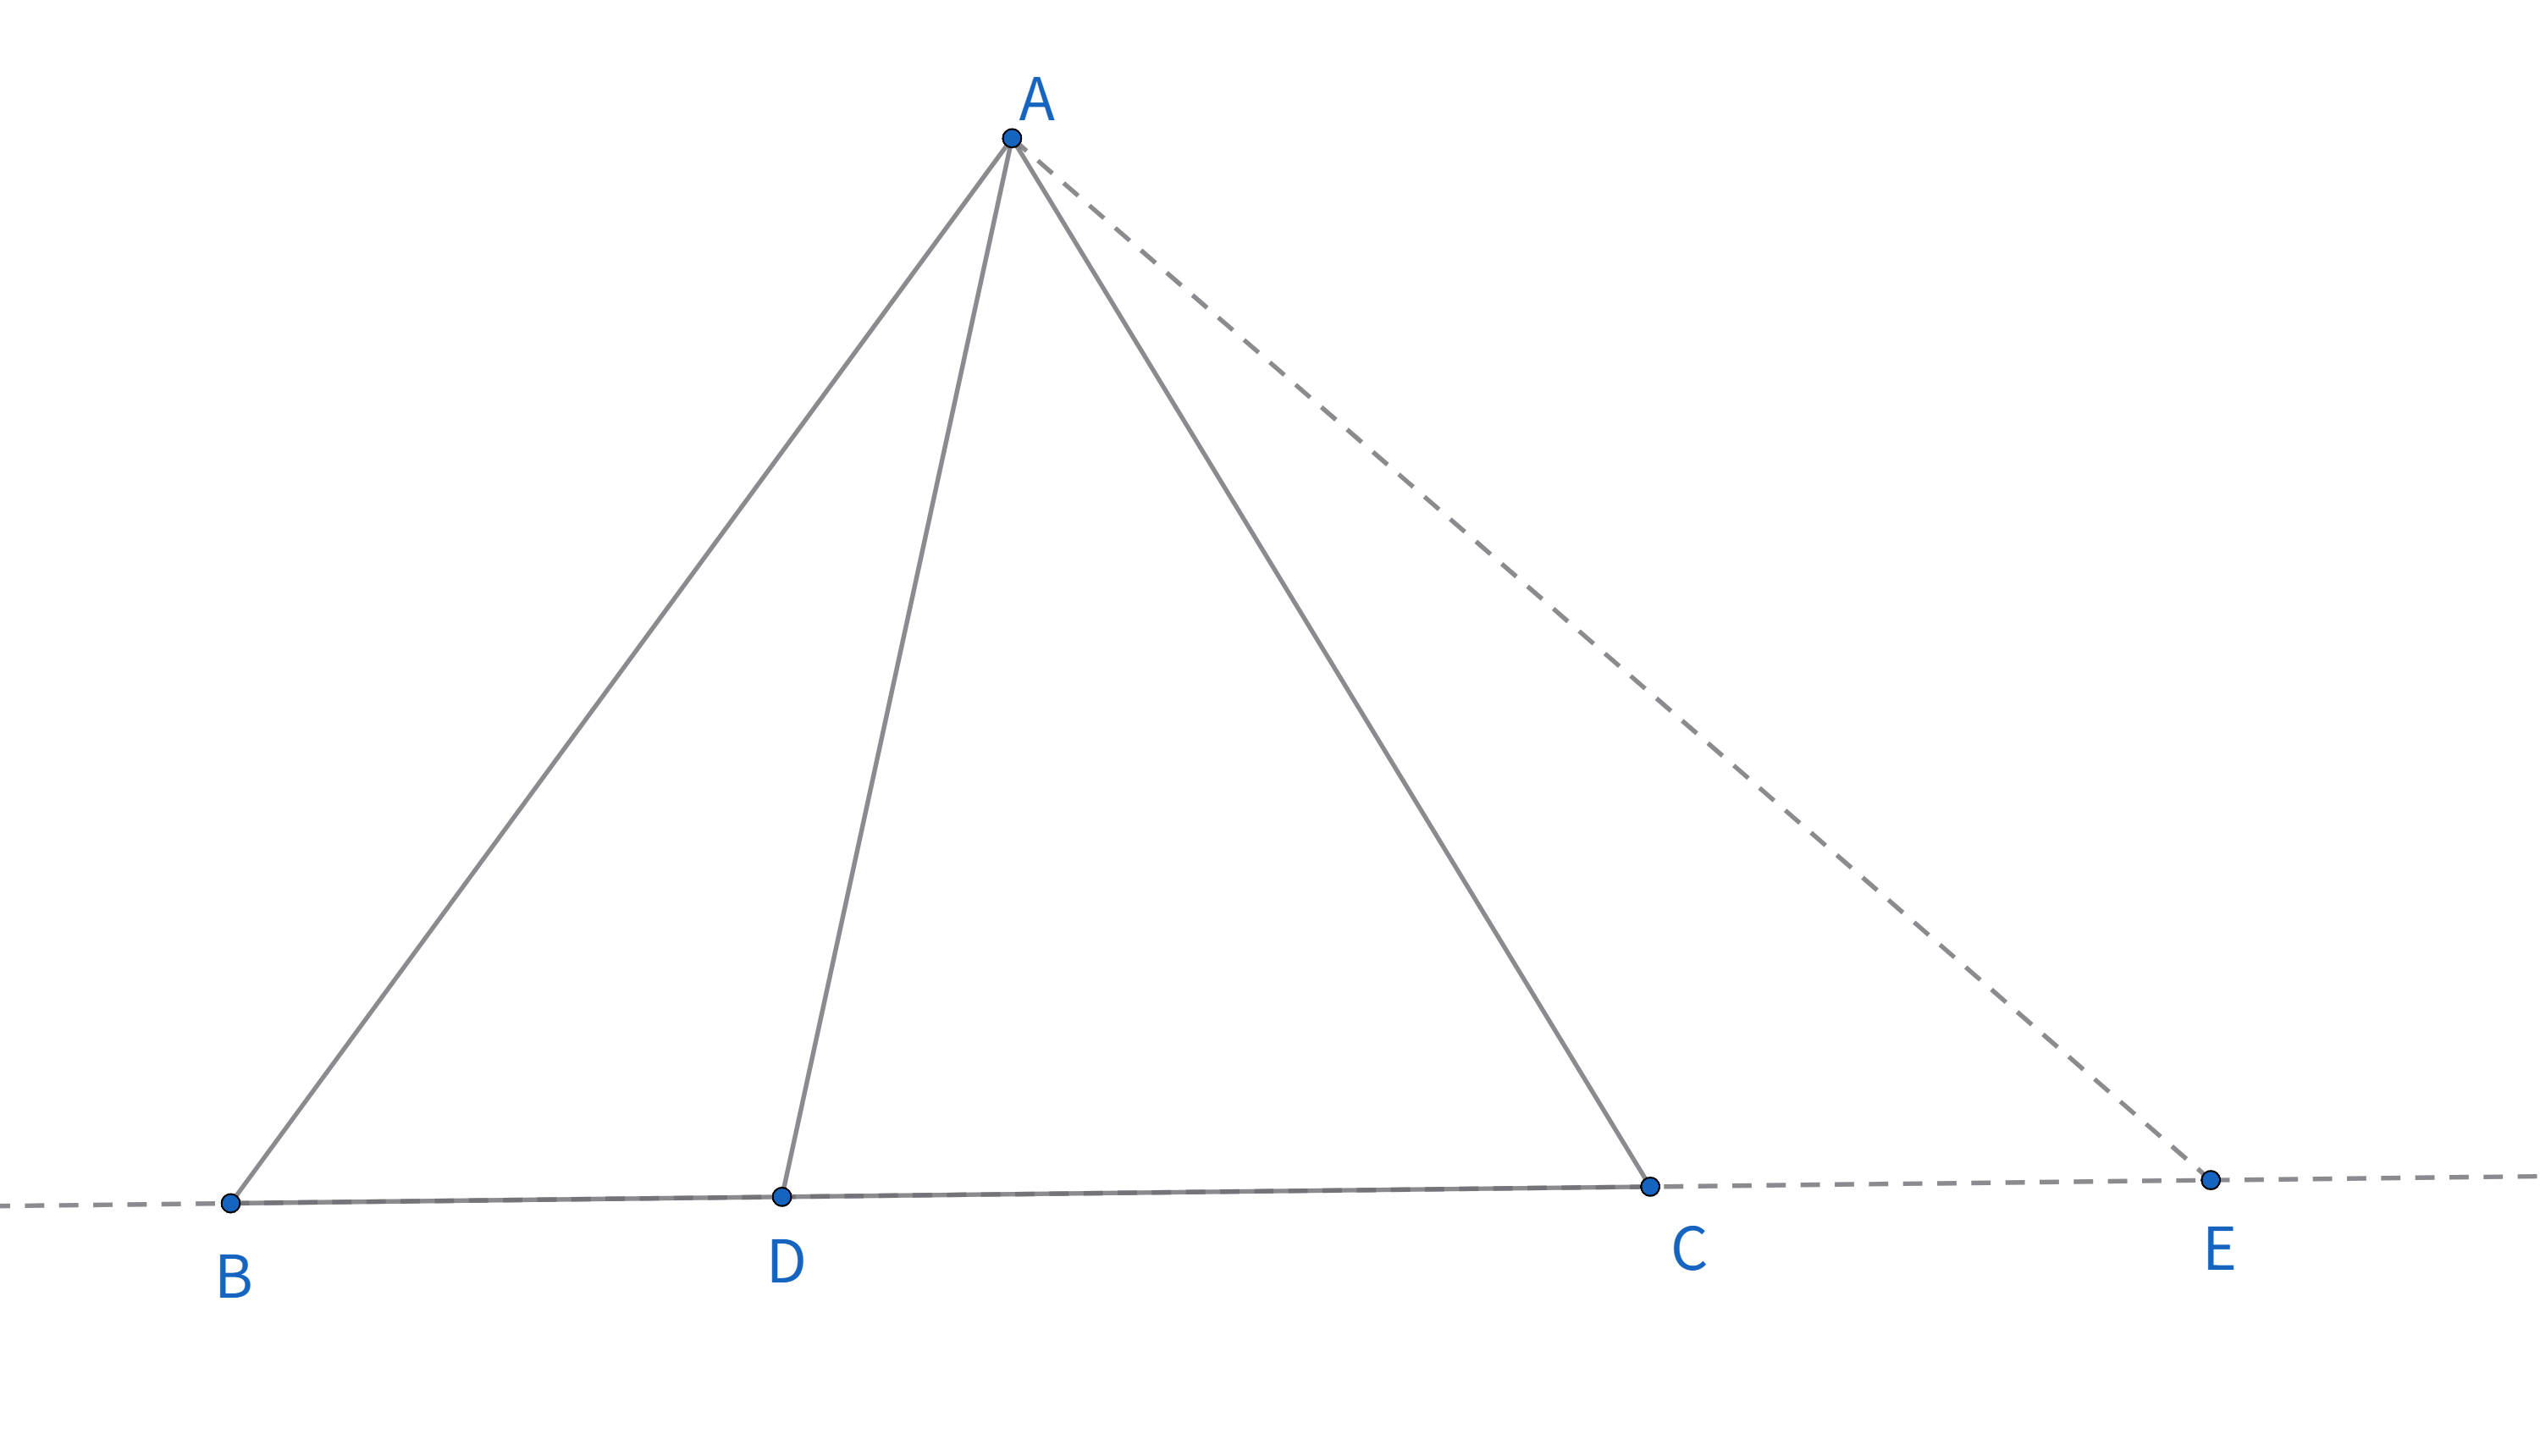
\includegraphics[width=0.7\linewidth]{figures/分角线定理.png}
    \caption{分角线定理}
\end{figure}
\begin{proposition}[角平分线定理]
在$\triangle ABC$中,$\angle A$的角平分线交BC边于D,则有
    $$
    \frac{BD}{DC} = \frac{AB}{AC}.
    $$
\end{proposition}

\begin{proposition}[中线定理]
    在$\triangle ABC$中,$\angle A$的角平分线交BC边于D,则有
    $$
    \frac{AC}{AB} = \frac{\sin \angle BAD}{\sin \angle CAD}.
    $$
\end{proposition}

\begin{figure}[htbp]
    \centering
    \hfill % 添加一些水平间距
    \begin{minipage}[t]{0.45\textwidth}
    \centering
    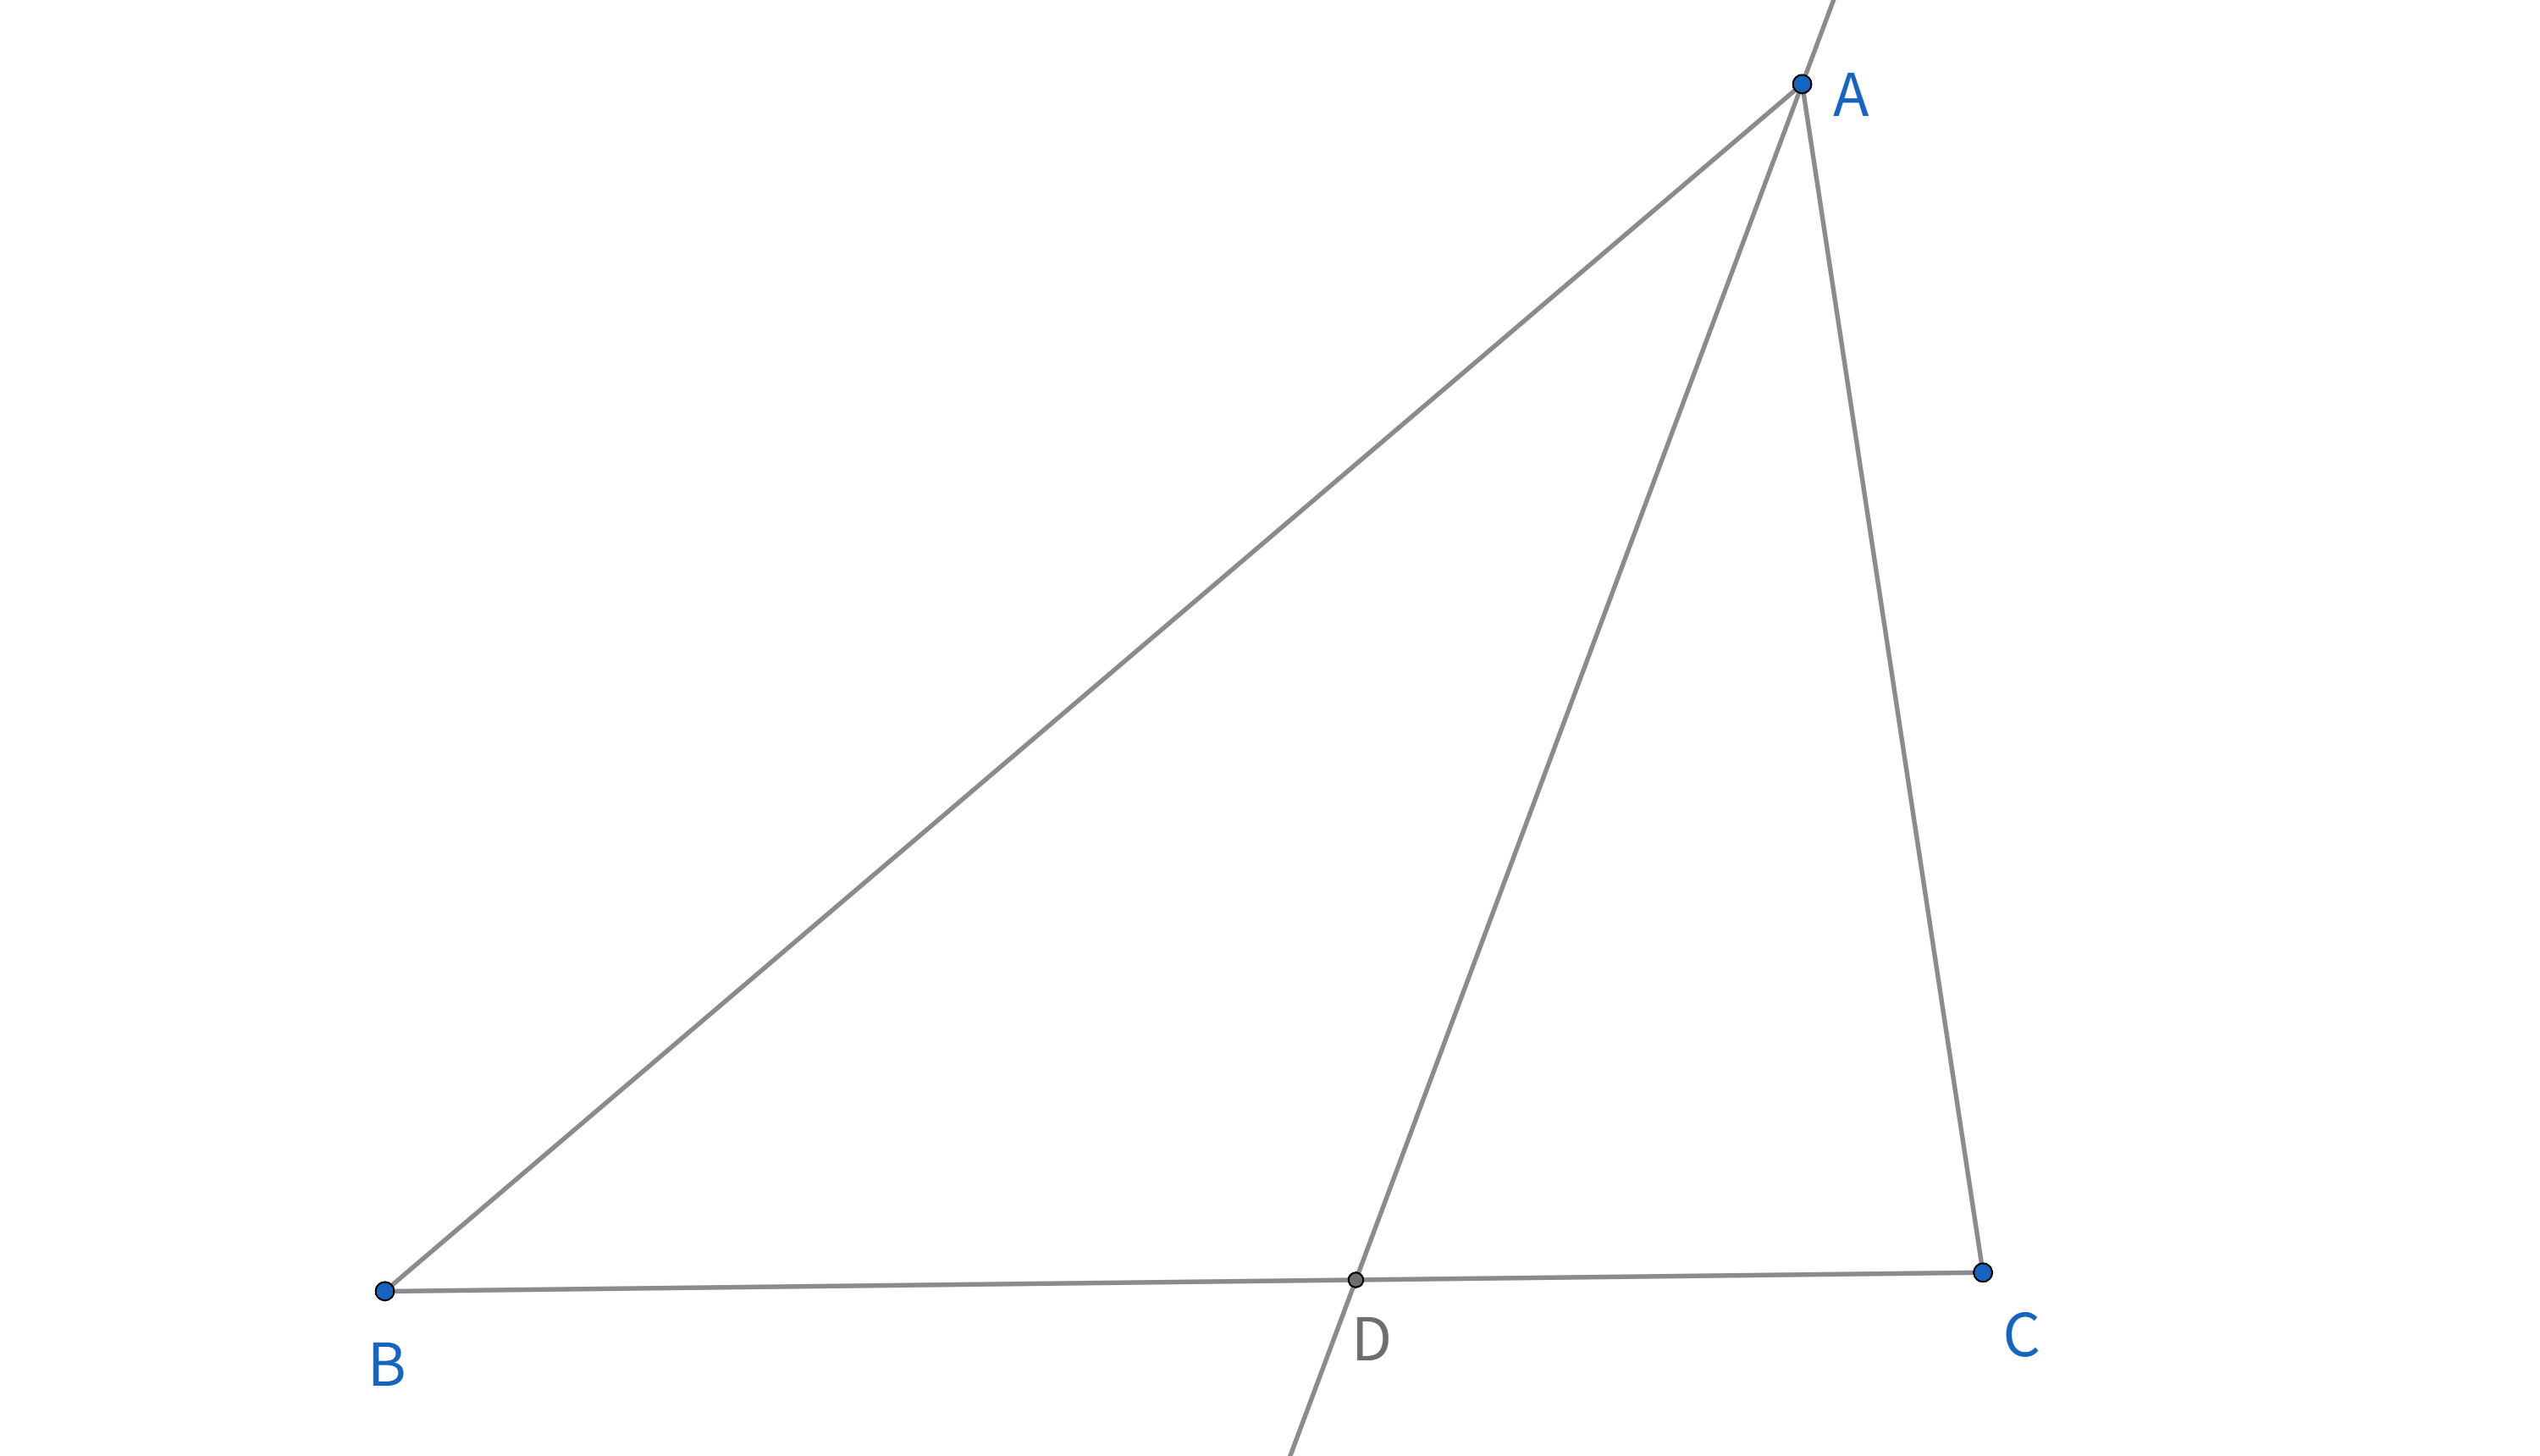
\includegraphics[width=\linewidth]{figures/分角线定理 -角平分线.png}
    \end{minipage}
    \hfill % 添加一些水平间距
    \begin{minipage}[t]{0.45\textwidth}
    \centering
    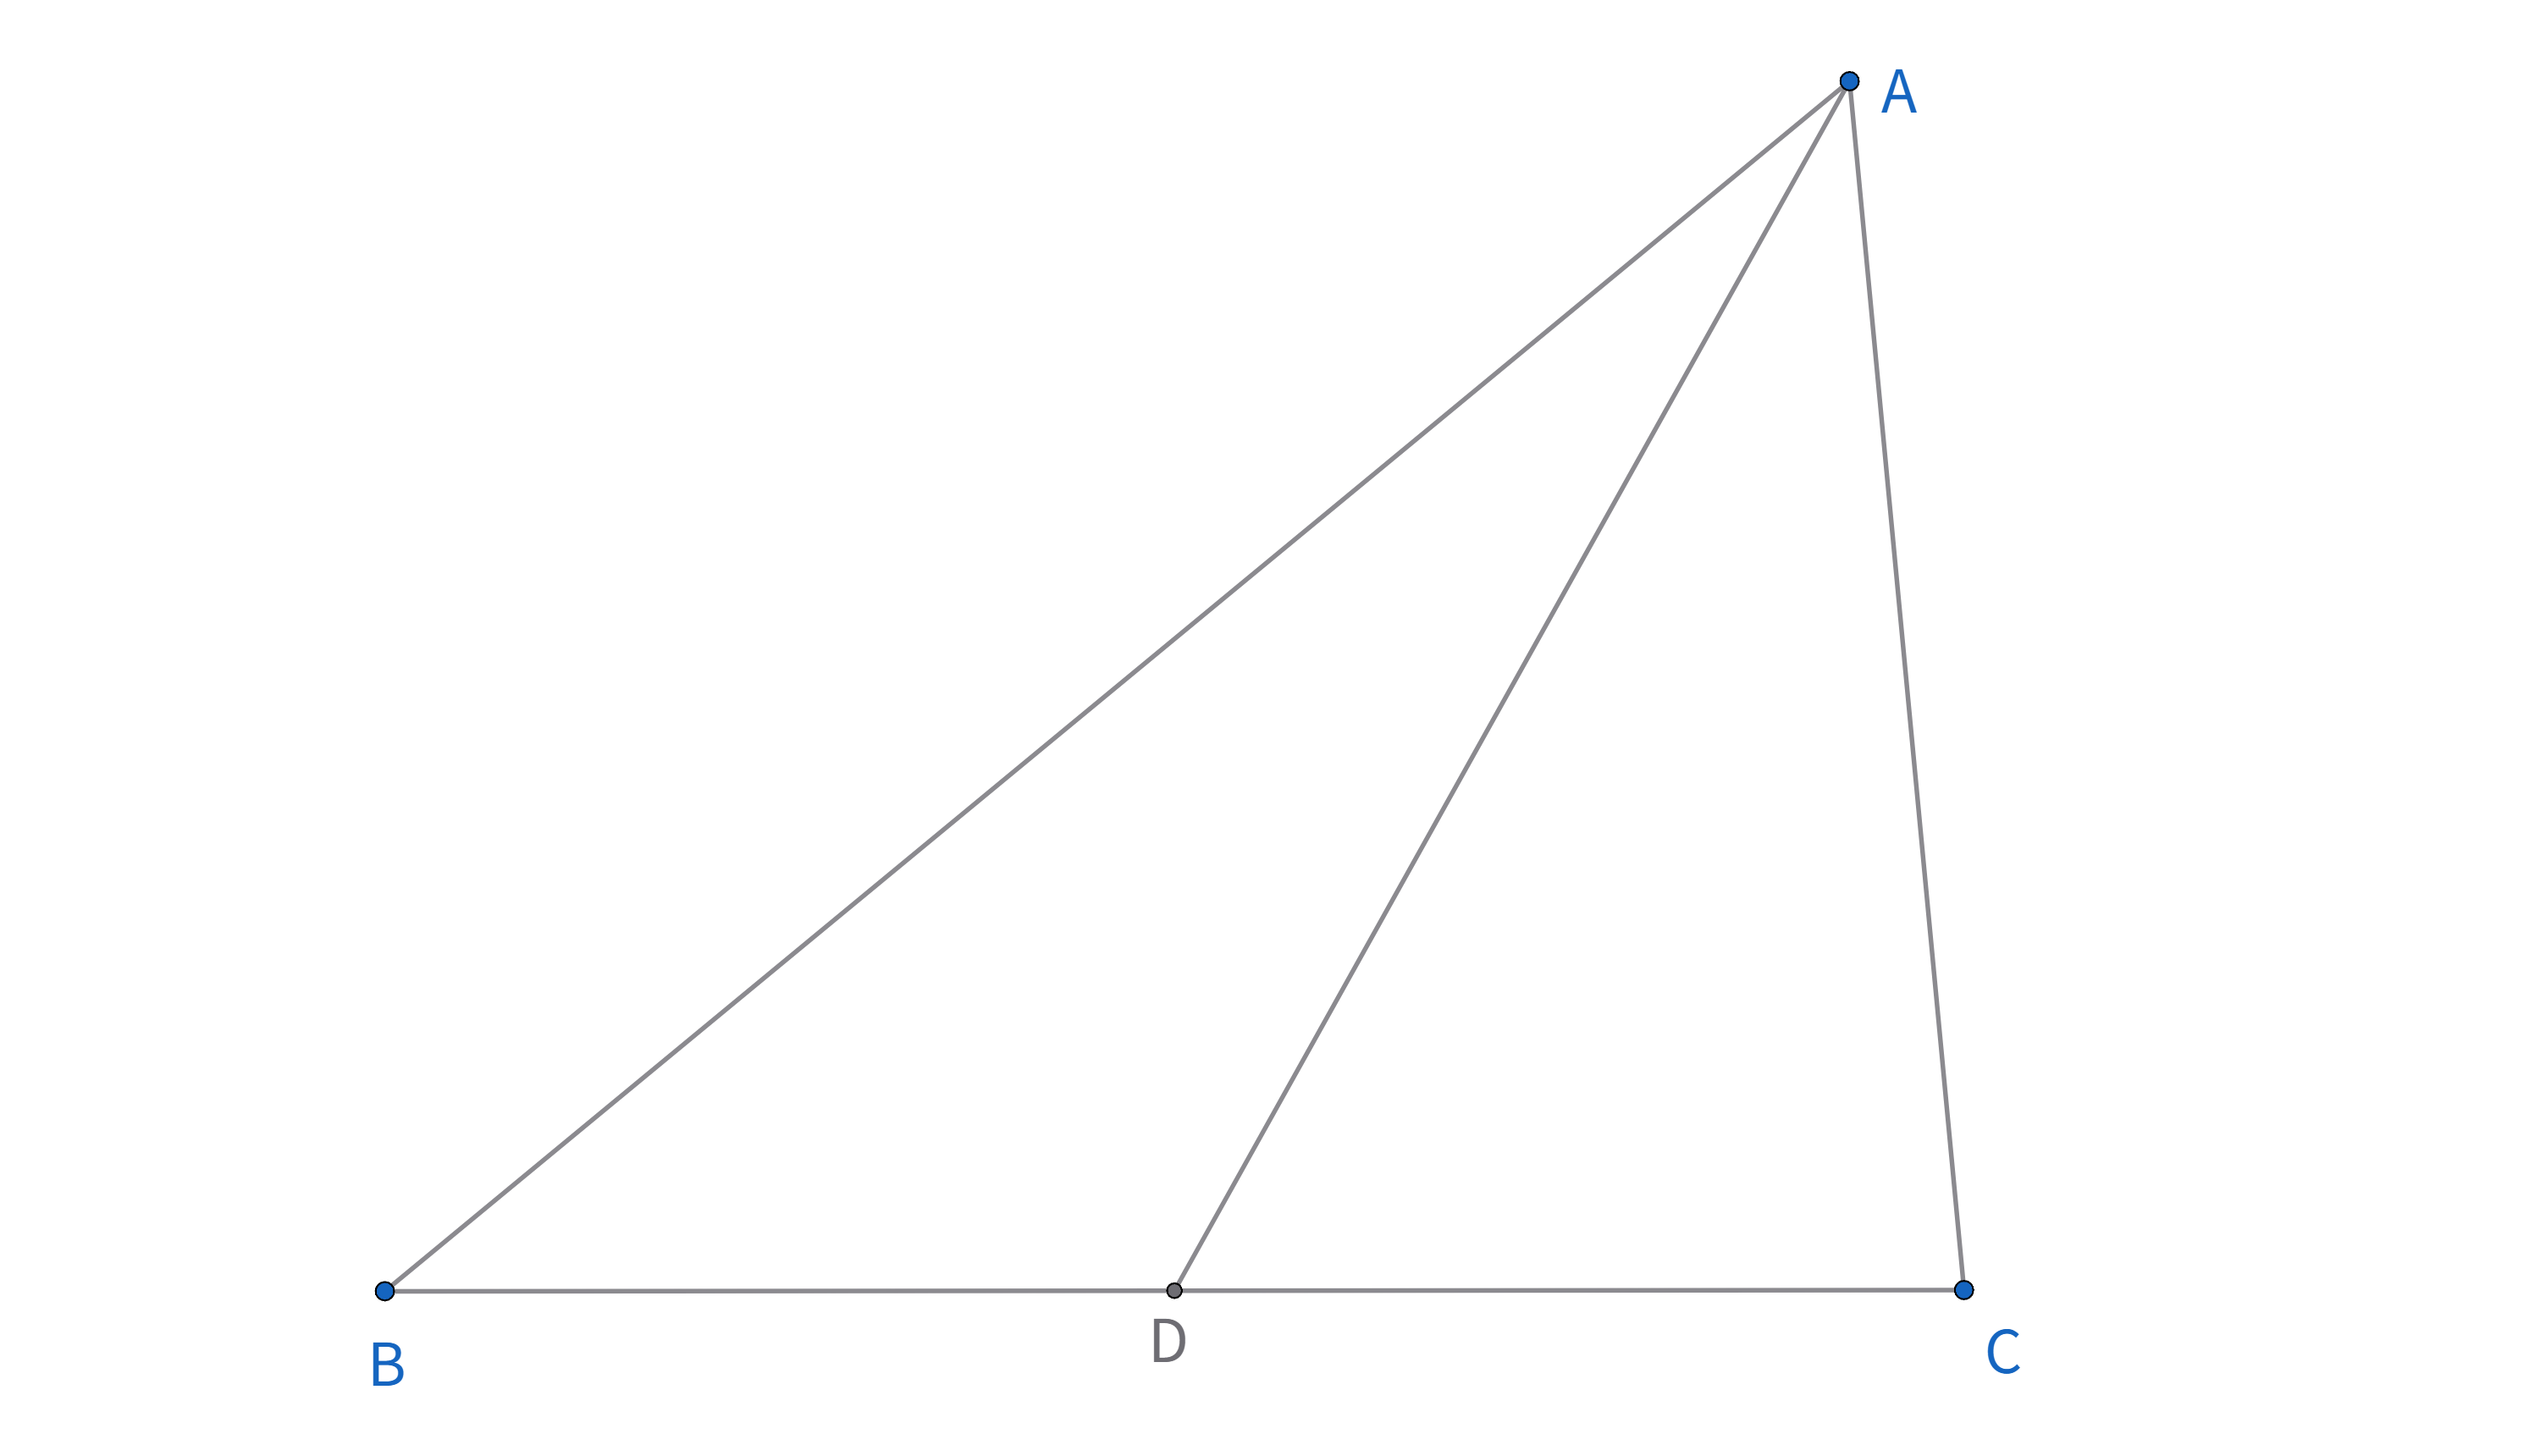
\includegraphics[width=\linewidth]{figures/分角线定理-中线.png}
    \end{minipage}
\end{figure}

\newpage 
\subsection{共边三角形}
\begin{proposition}
    $\triangle ABC,\triangle ABD$共用BC边,有下列等式成立:
    $$
    \frac{\sin\angle BAC}{\sin\angle BAD} = \frac{BC}{BD}\cdot \frac{\sin\angle ACB}{\sin\angle ADB}.
    $$
\end{proposition}
\begin{figure}[ht]
    \centering
    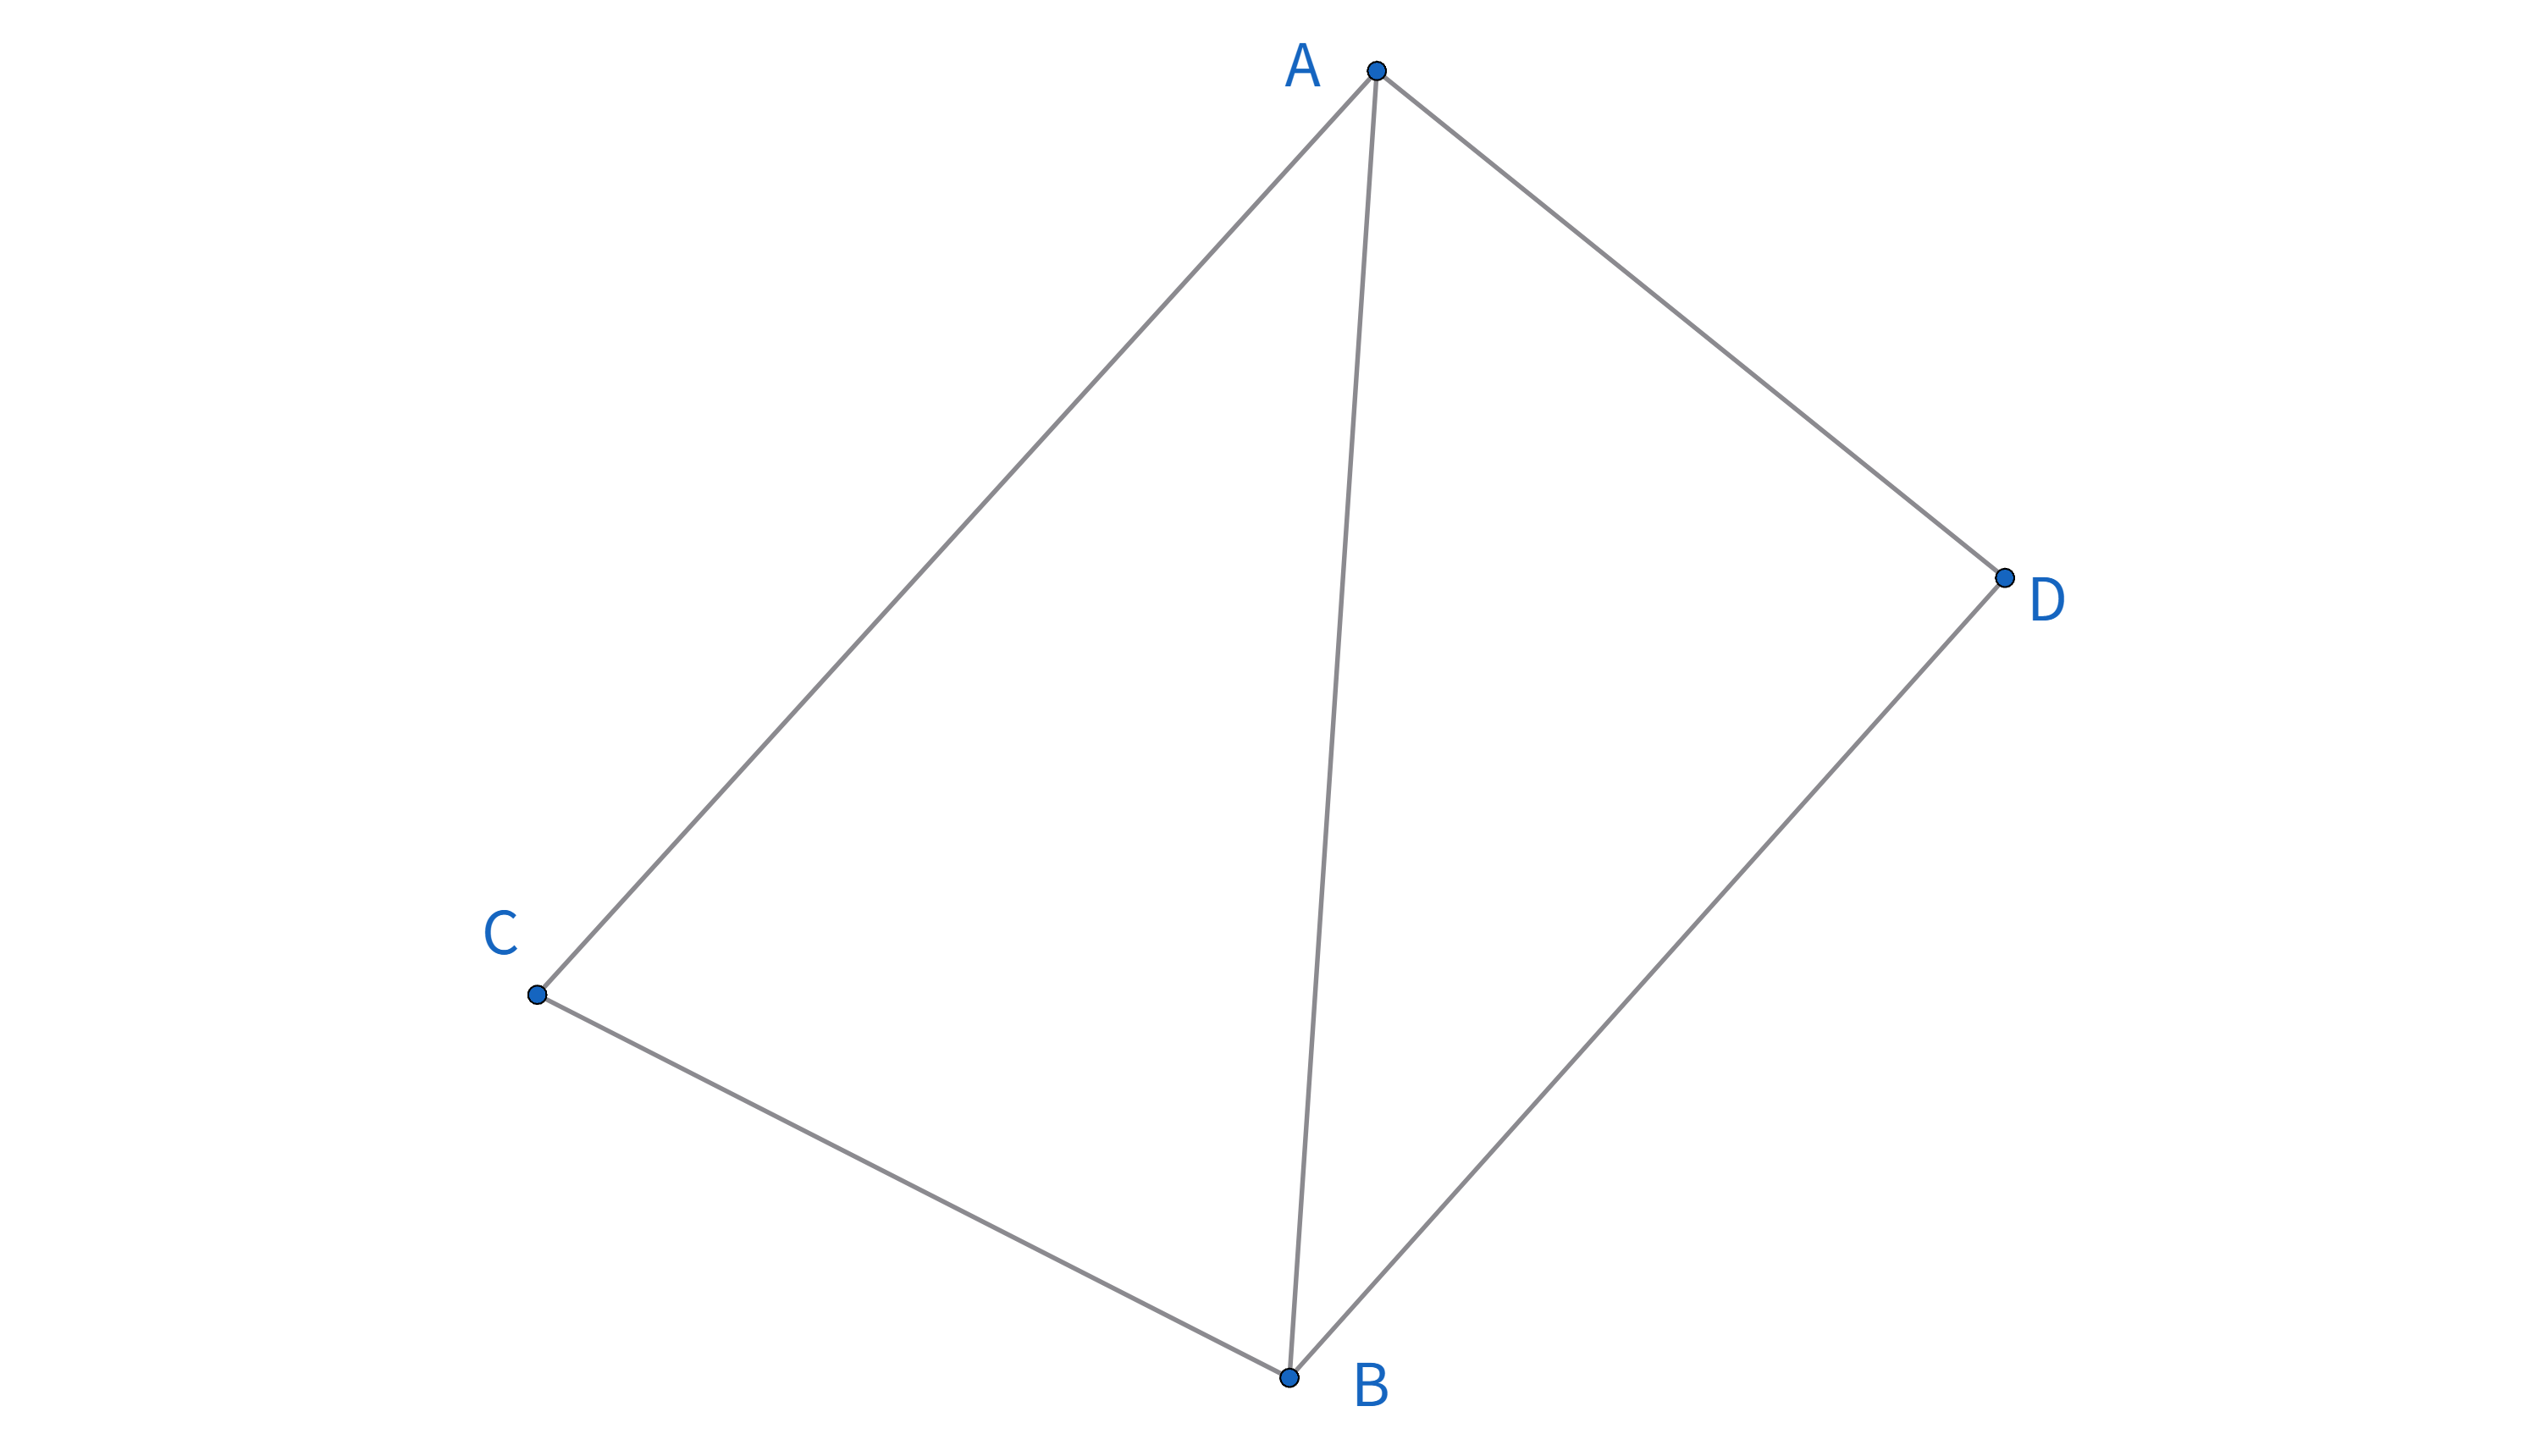
\includegraphics[width=0.7\linewidth]{figures/共边三角形.png}
    \caption{共边三角形}
\end{figure}



\newpage 
\subsection{托勒密(Ptolemy)定理}
\begin{theorem}[托勒密定理]
    圆的内接四边形对角线乘积等于两组对边乘积之和。
    $$AC \cdot BD = AB \cdot CD + BC \cdot AD.$$
\end{theorem}
\begin{figure}[ht]
    \centering
    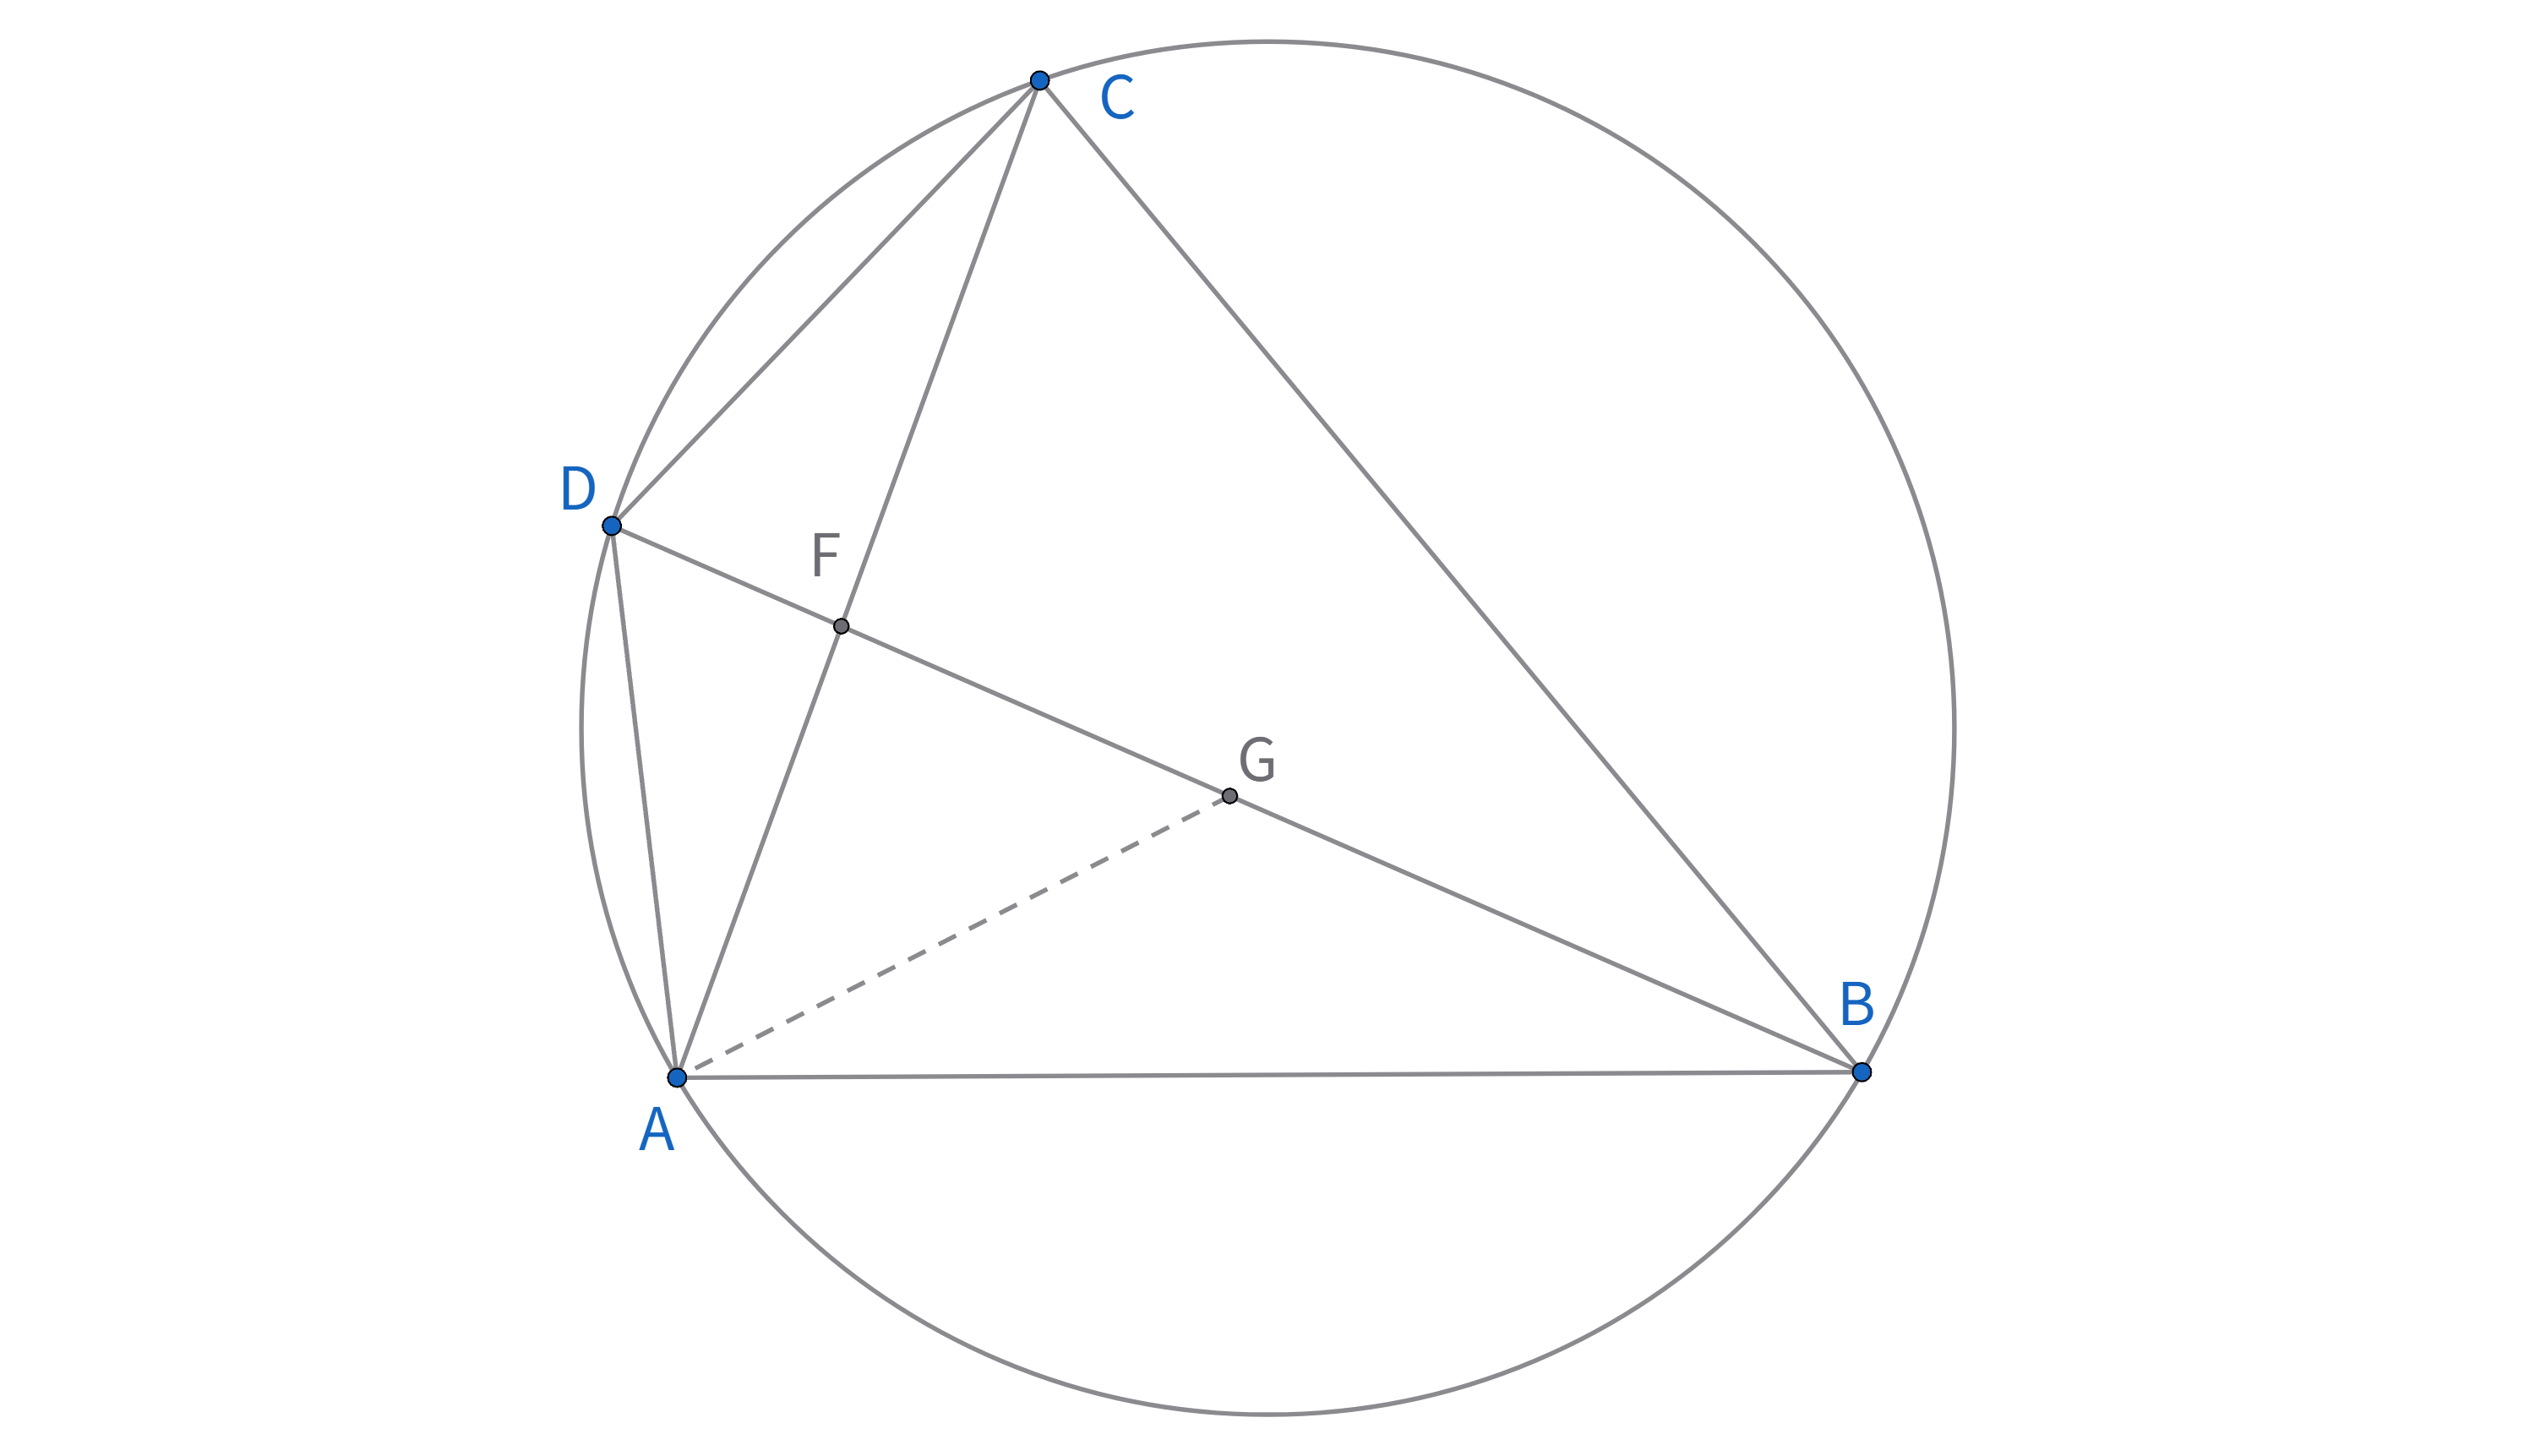
\includegraphics[width=0.7\linewidth]{figures/托勒密定理.png}
    \caption{托勒密定理}
\end{figure}

\subsubsection{三弦定理}
\begin{theorem}[三弦定理]
    如果A是圆上任意一点,AB、ACAD是该圆上顺次的三条弦,则
    $$
    AC\cdot \sin \angle BAD = AB\cdot \sin \angle CAD+AD\cdot \sin \angle CAB
    $$
\end{theorem}

\newpage 
\subsubsection{直线上的托勒密定理}
\begin{theorem}[直线上的托勒密定理]
    若A、B、C、D为一条直线上依次排列的四点,则
    $$AC \cdot BD = AB \cdot CD + BC \cdot AD.$$
\end{theorem}
\subsubsection{托勒密不等式}
\begin{theorem}[托勒密不等式]
    ABCD为任意凸四边形,则
    $$AB \cdot CD + BC \cdot AD\leq AC \cdot BD.$$
    当且仅当ABCD四点共圆时取得等号。
\end{theorem}
\begin{figure}[htbp]
    \centering
    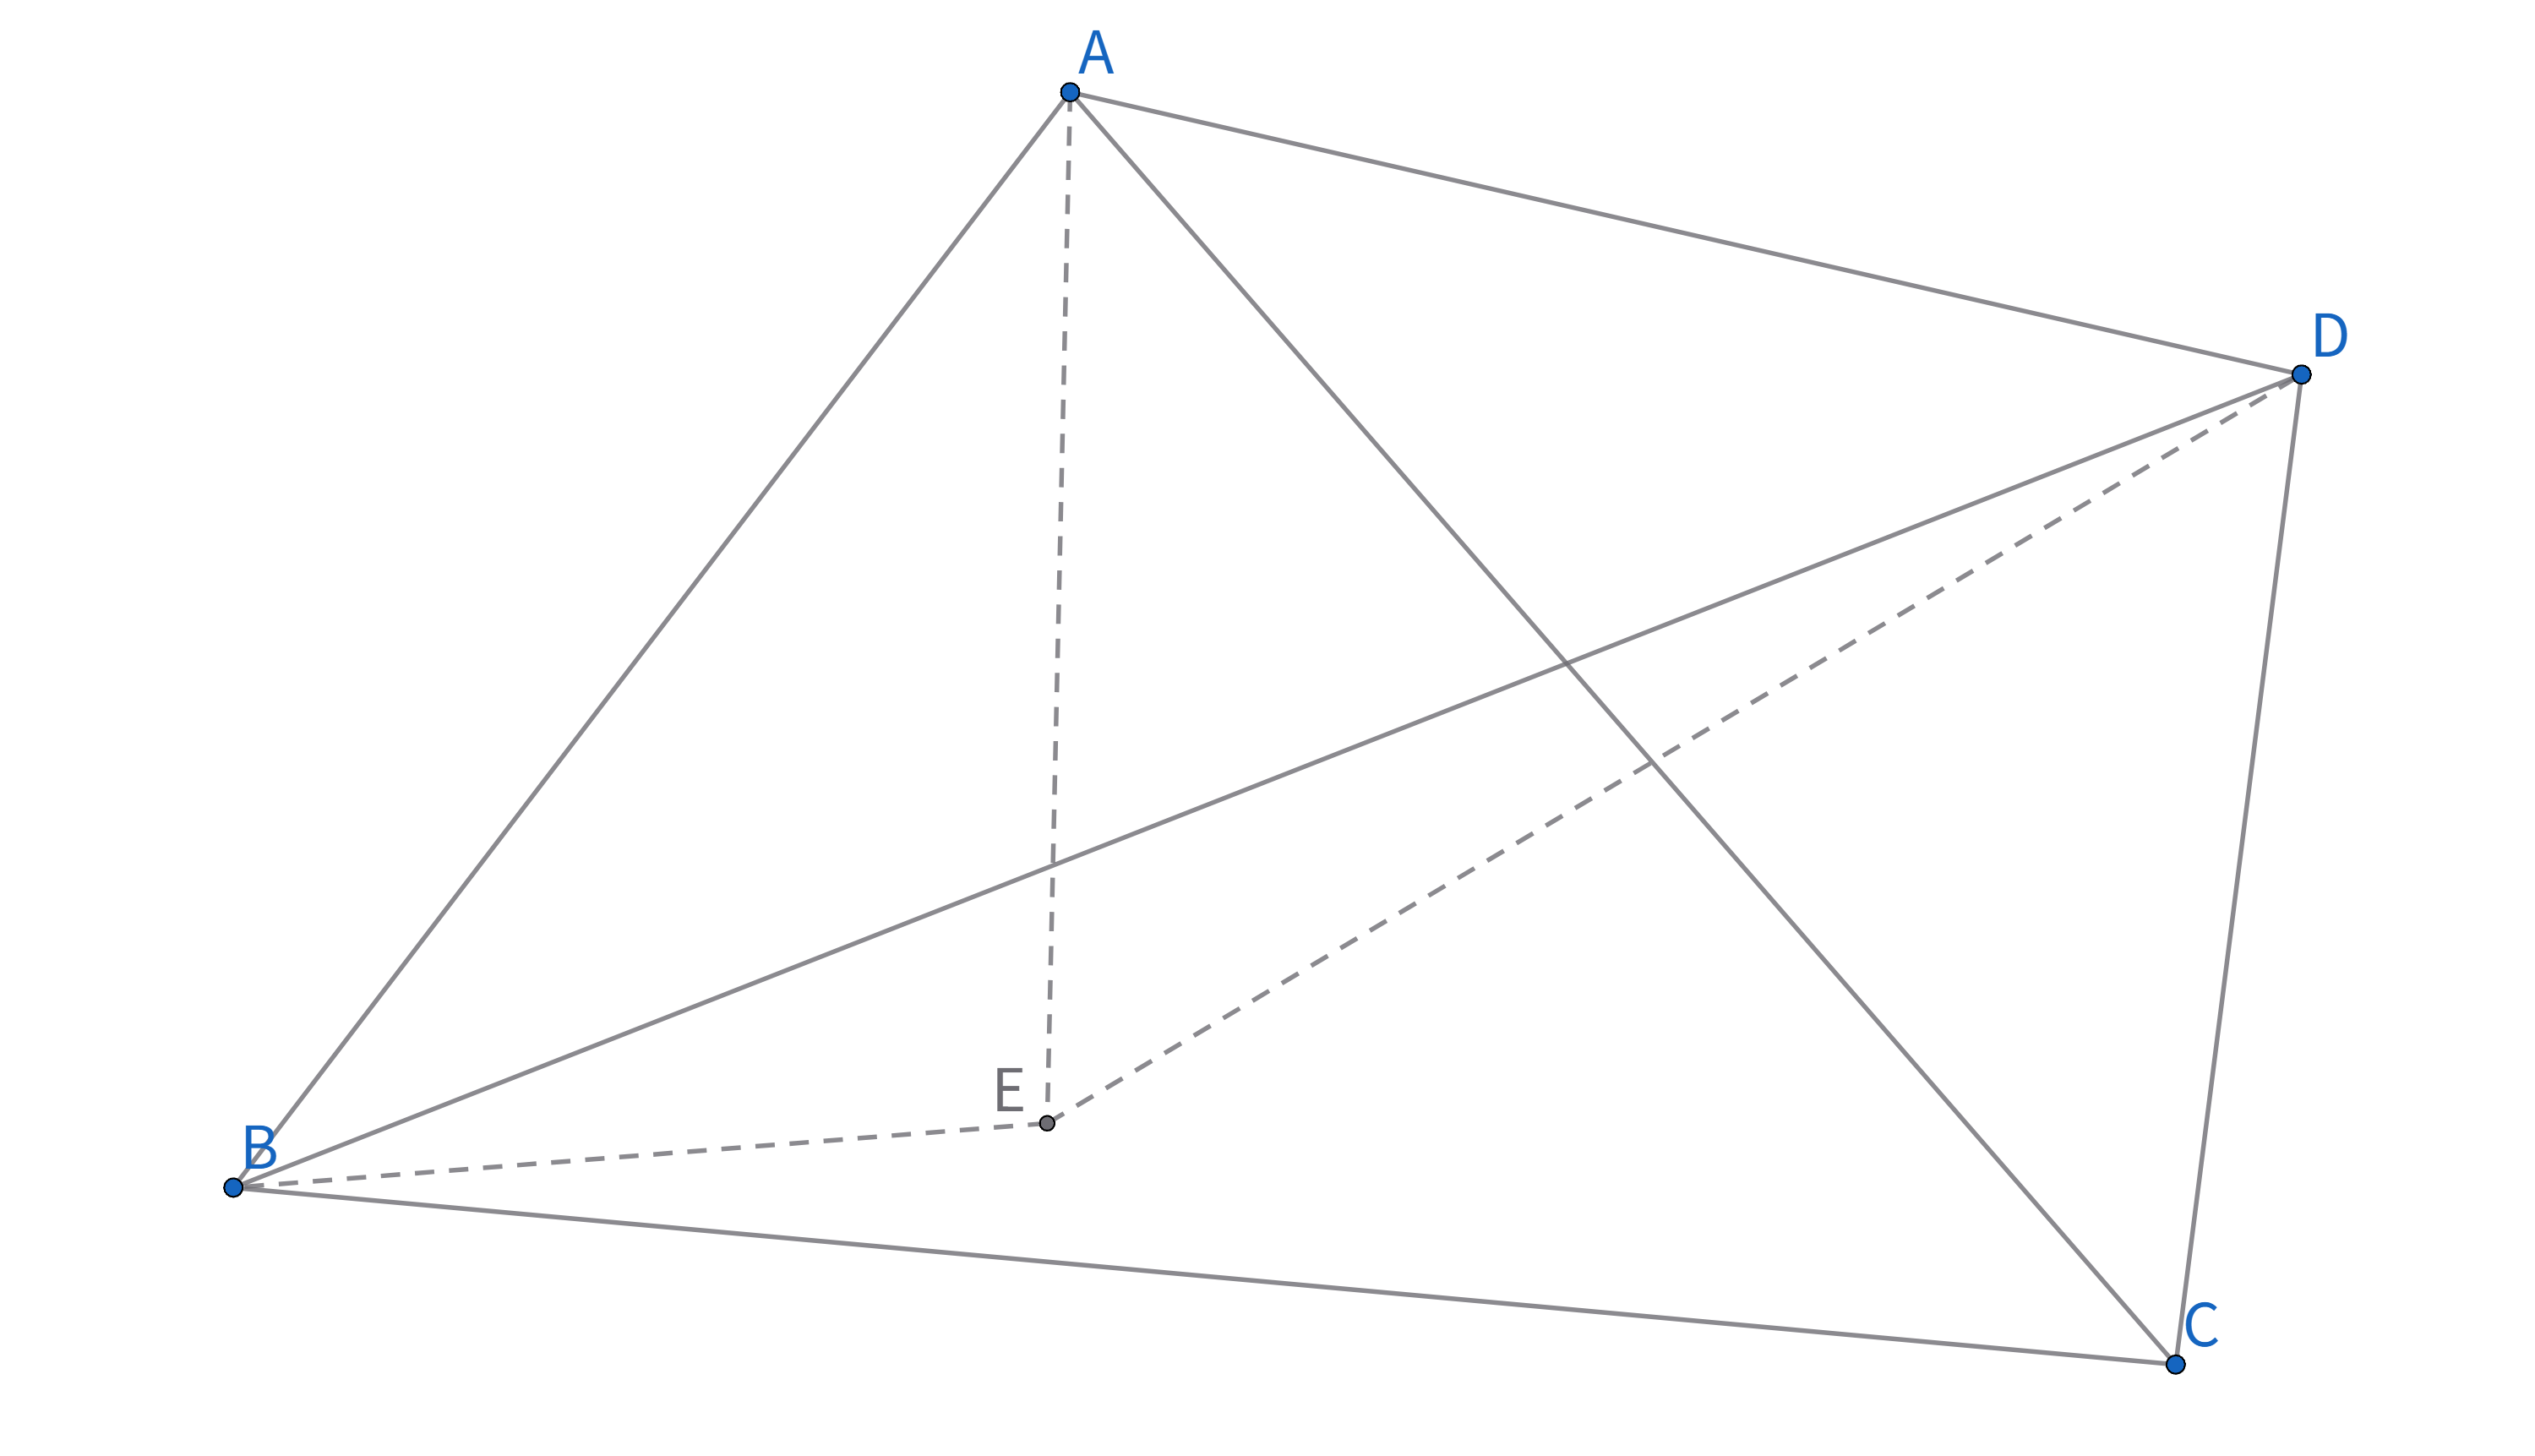
\includegraphics[width=0.7\linewidth]{figures/托勒密不等式.png}
    \caption{托勒密不等式}
\end{figure}

\newpage 
\subsection{斯特瓦尔特(Stewart)定理}
\begin{theorem}[斯特瓦尔特定理]
    B、P、C依次分别为A点引出的三条射线上的点,则等式
    $$
    AB^2\cdot PC+AC^2\cdot PB = AP^2\cdot BC + PB\cdot PC\cdot BC.
    $$
    等价于B、P、C三点共线。
\end{theorem}
\begin{figure}[ht]
    \centering
    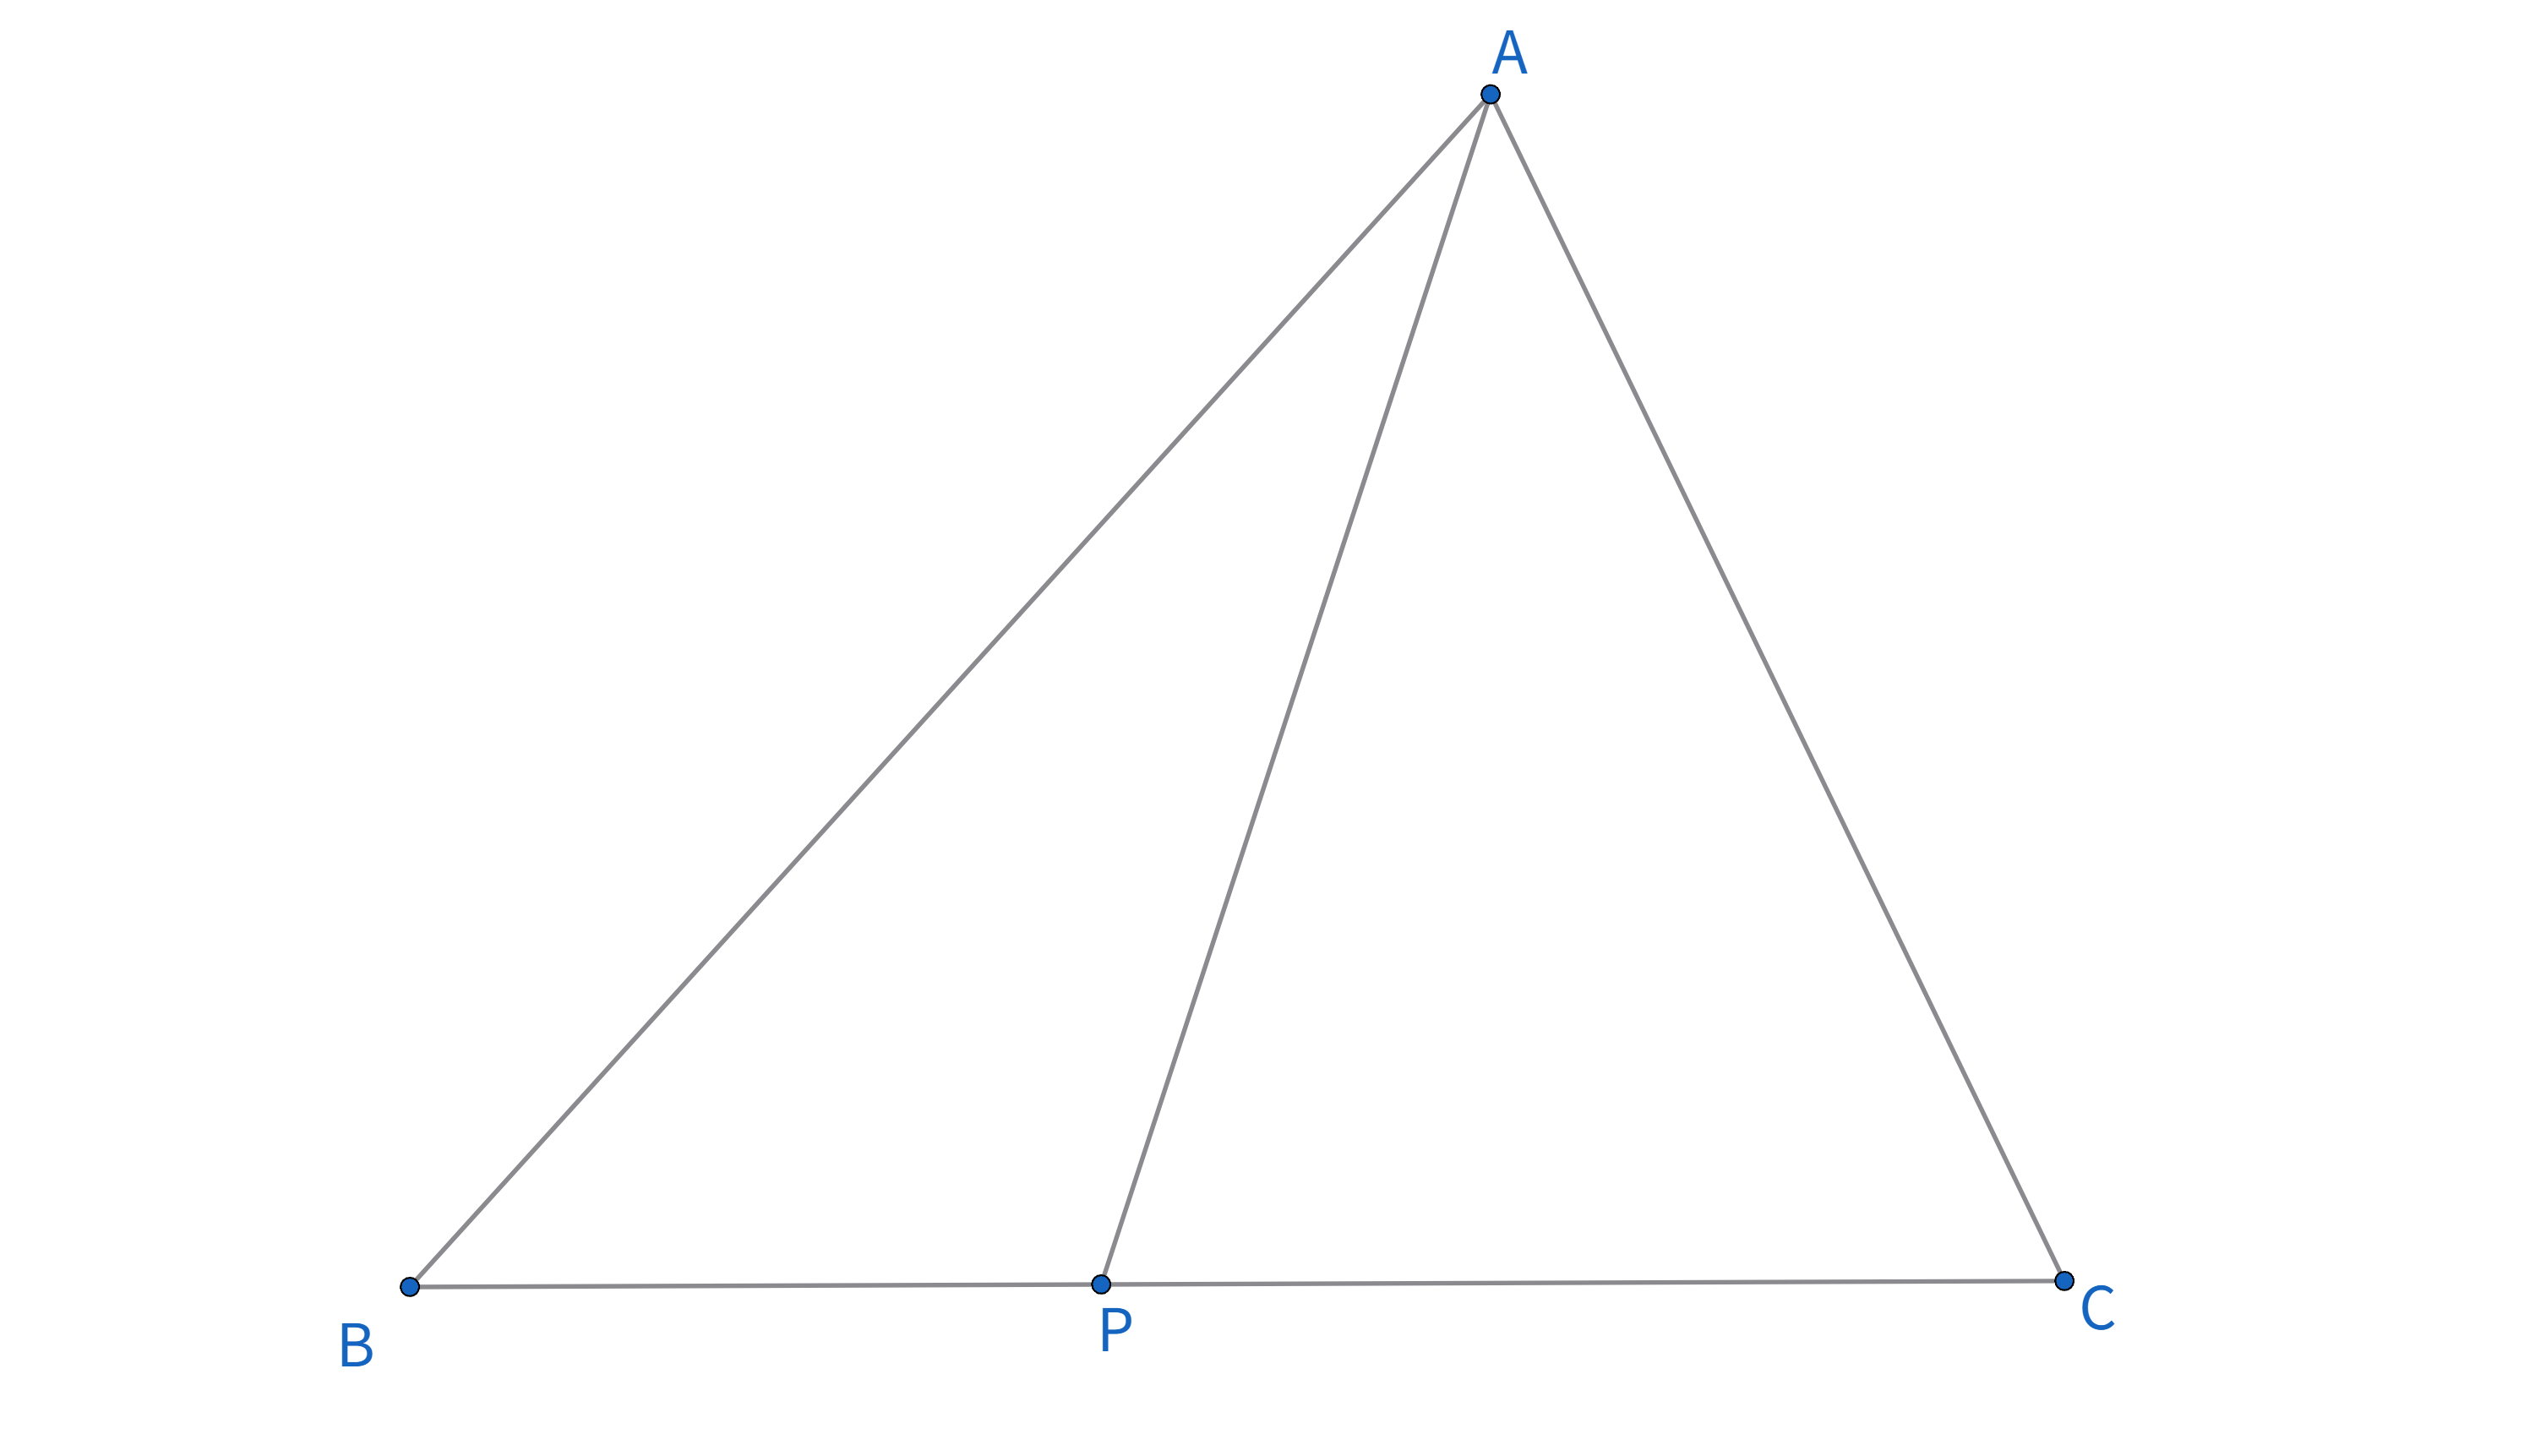
\includegraphics[width=0.7\linewidth]{figures/斯特瓦尔特定理.png}
    \caption{斯特瓦尔特定理}
\end{figure}


\newpage
\subsection{定差幂线}
\begin{theorem}[定差幂线定理]
    设MN、PQ是两条线段,则$MN\perp PQ$的充分必要条件是
    $$PM^2-PN^2 = QM^2-QN^2$$.
\end{theorem}
\begin{figure}[ht]
    \centering
    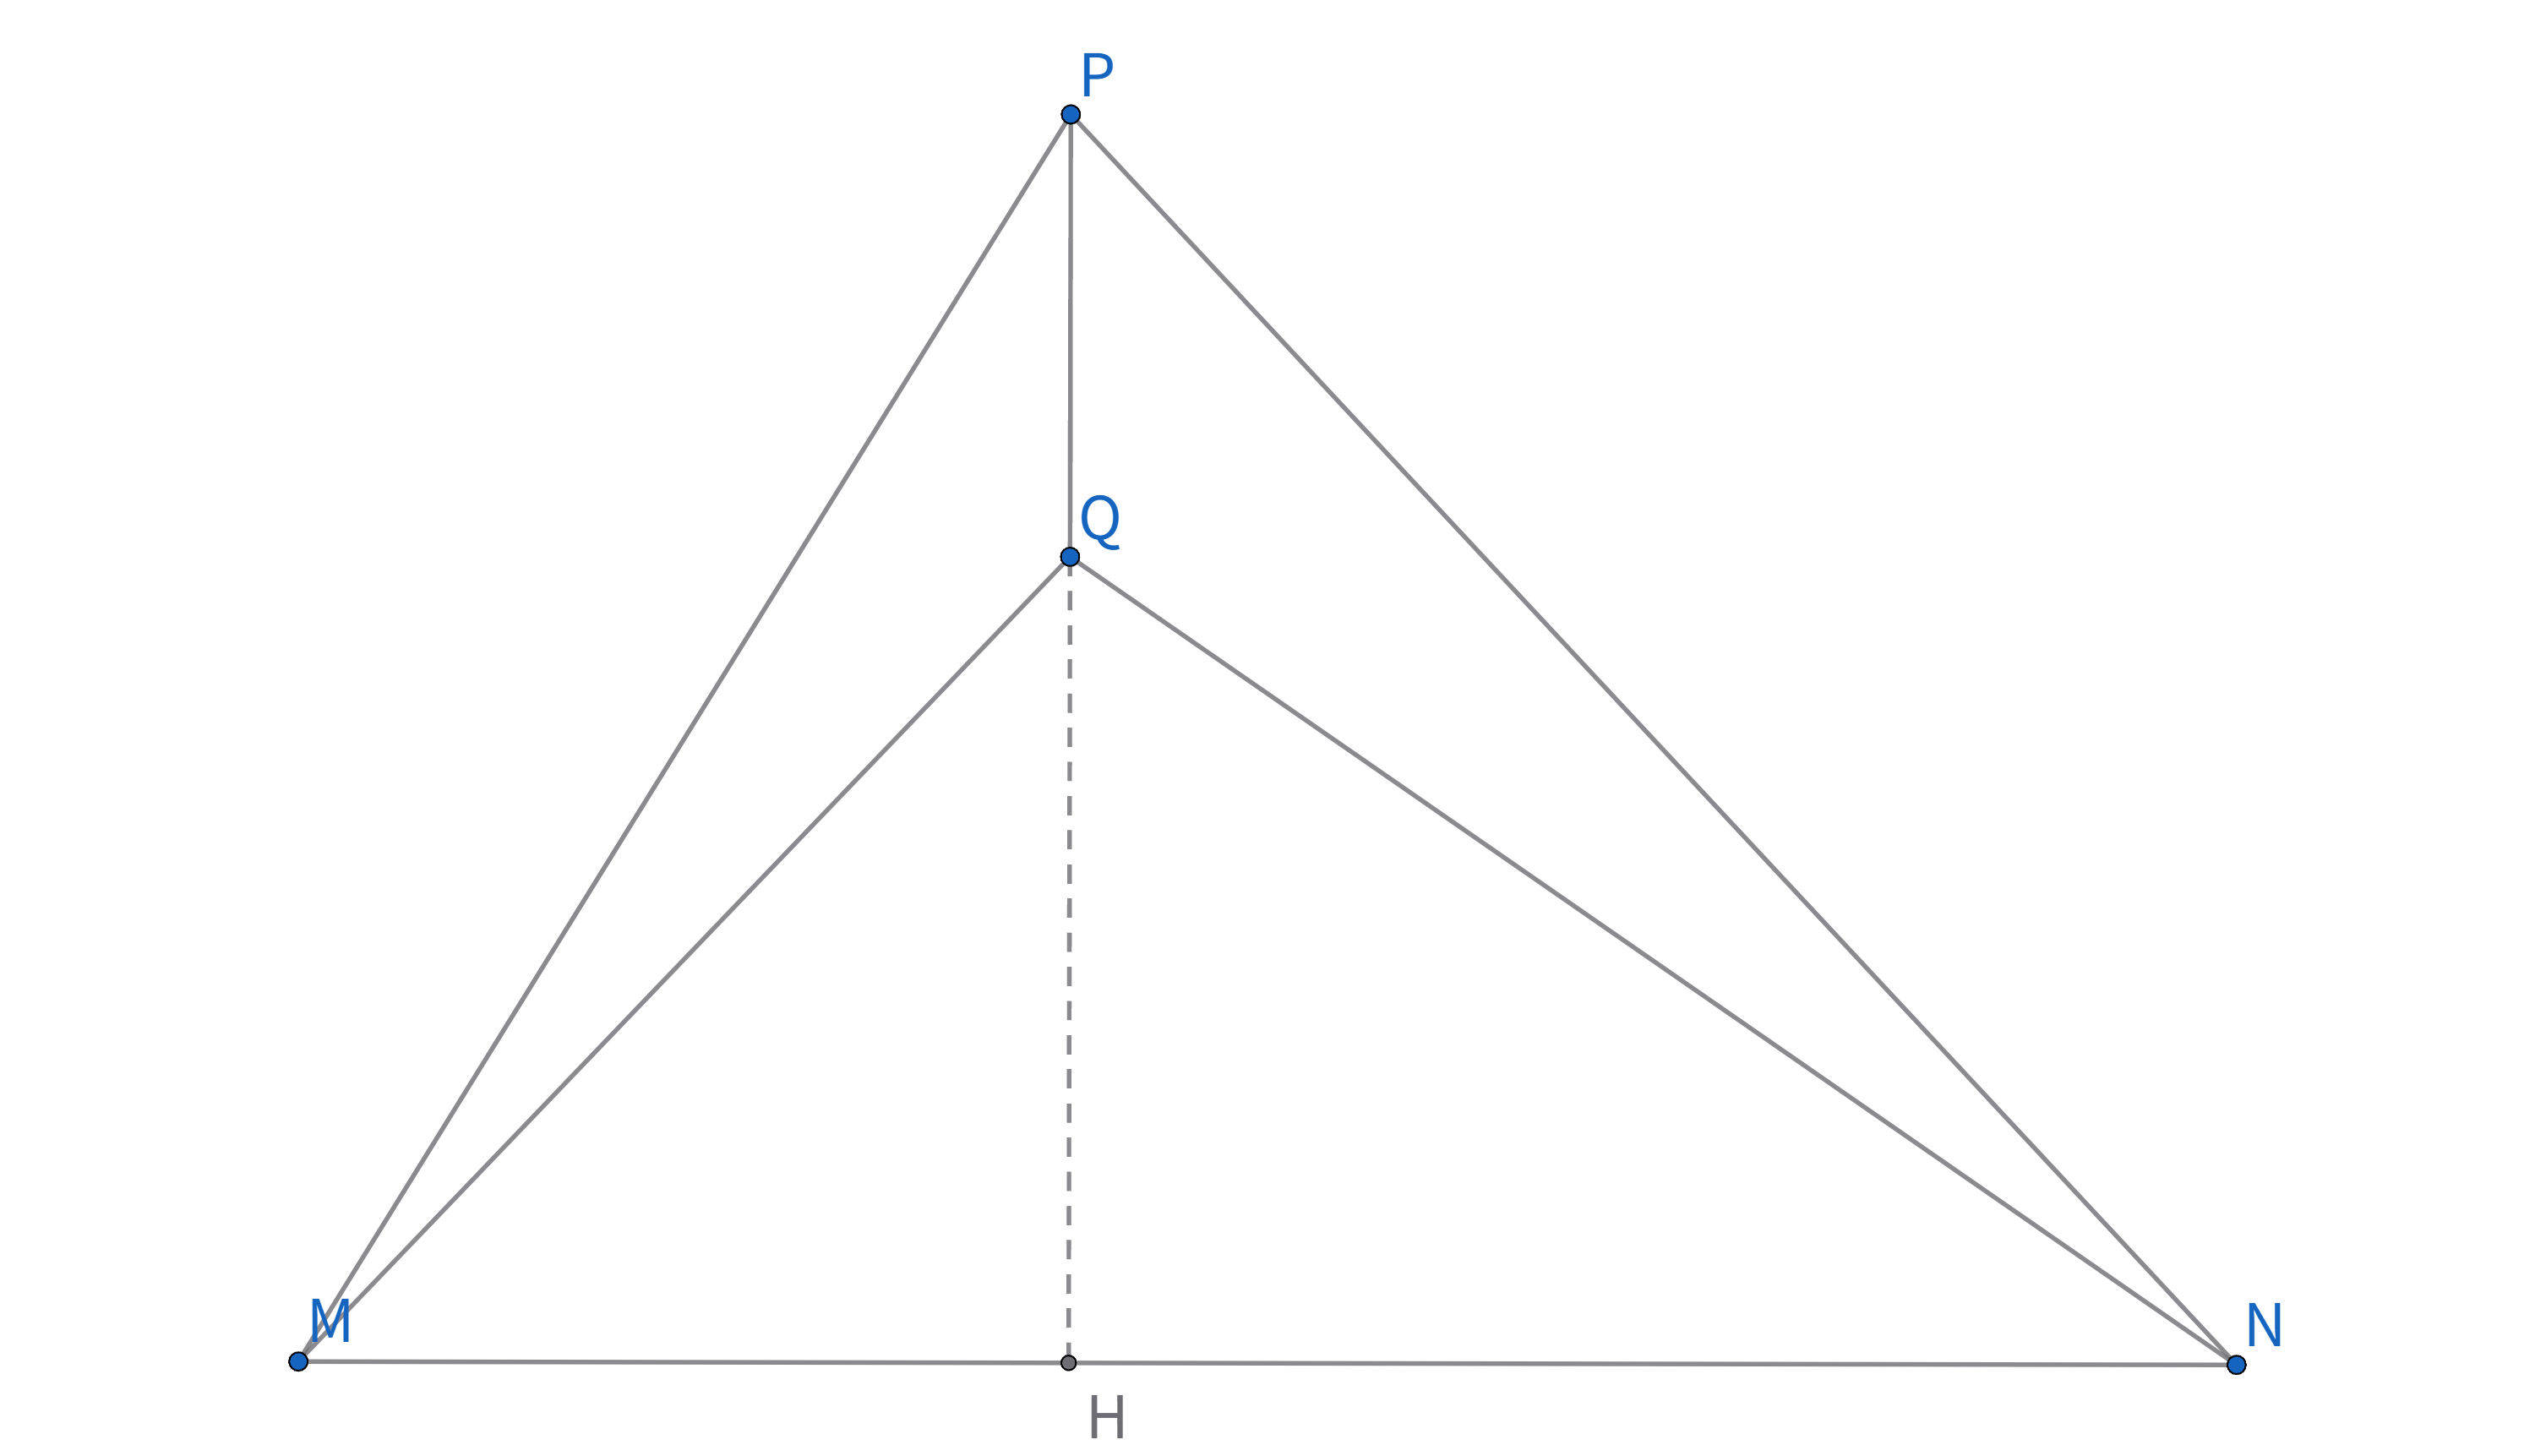
\includegraphics[width=0.7\linewidth]{figures/定差幂线.png}
    \caption{定差幂线}
\end{figure}


\newpage 
\subsection{张角定理}
\begin{theorem}[张角(Spread Angle)定理]
    A、C、B依次分别是平面内一点P所引三条射线上的点,AC、CB对P的张角分别为$\alpha,\beta$,并且$\alpha+\beta<180^circ$,则A、C、B共线的充分必要条件是
    $$
    \frac{\sin(\alpha+\beta)}{PC}
    = \frac{\sin\alpha}{PB}
    +\frac{\sin\beta}{PA}.
    $$
\end{theorem}
\begin{figure}[ht]
    \centering
    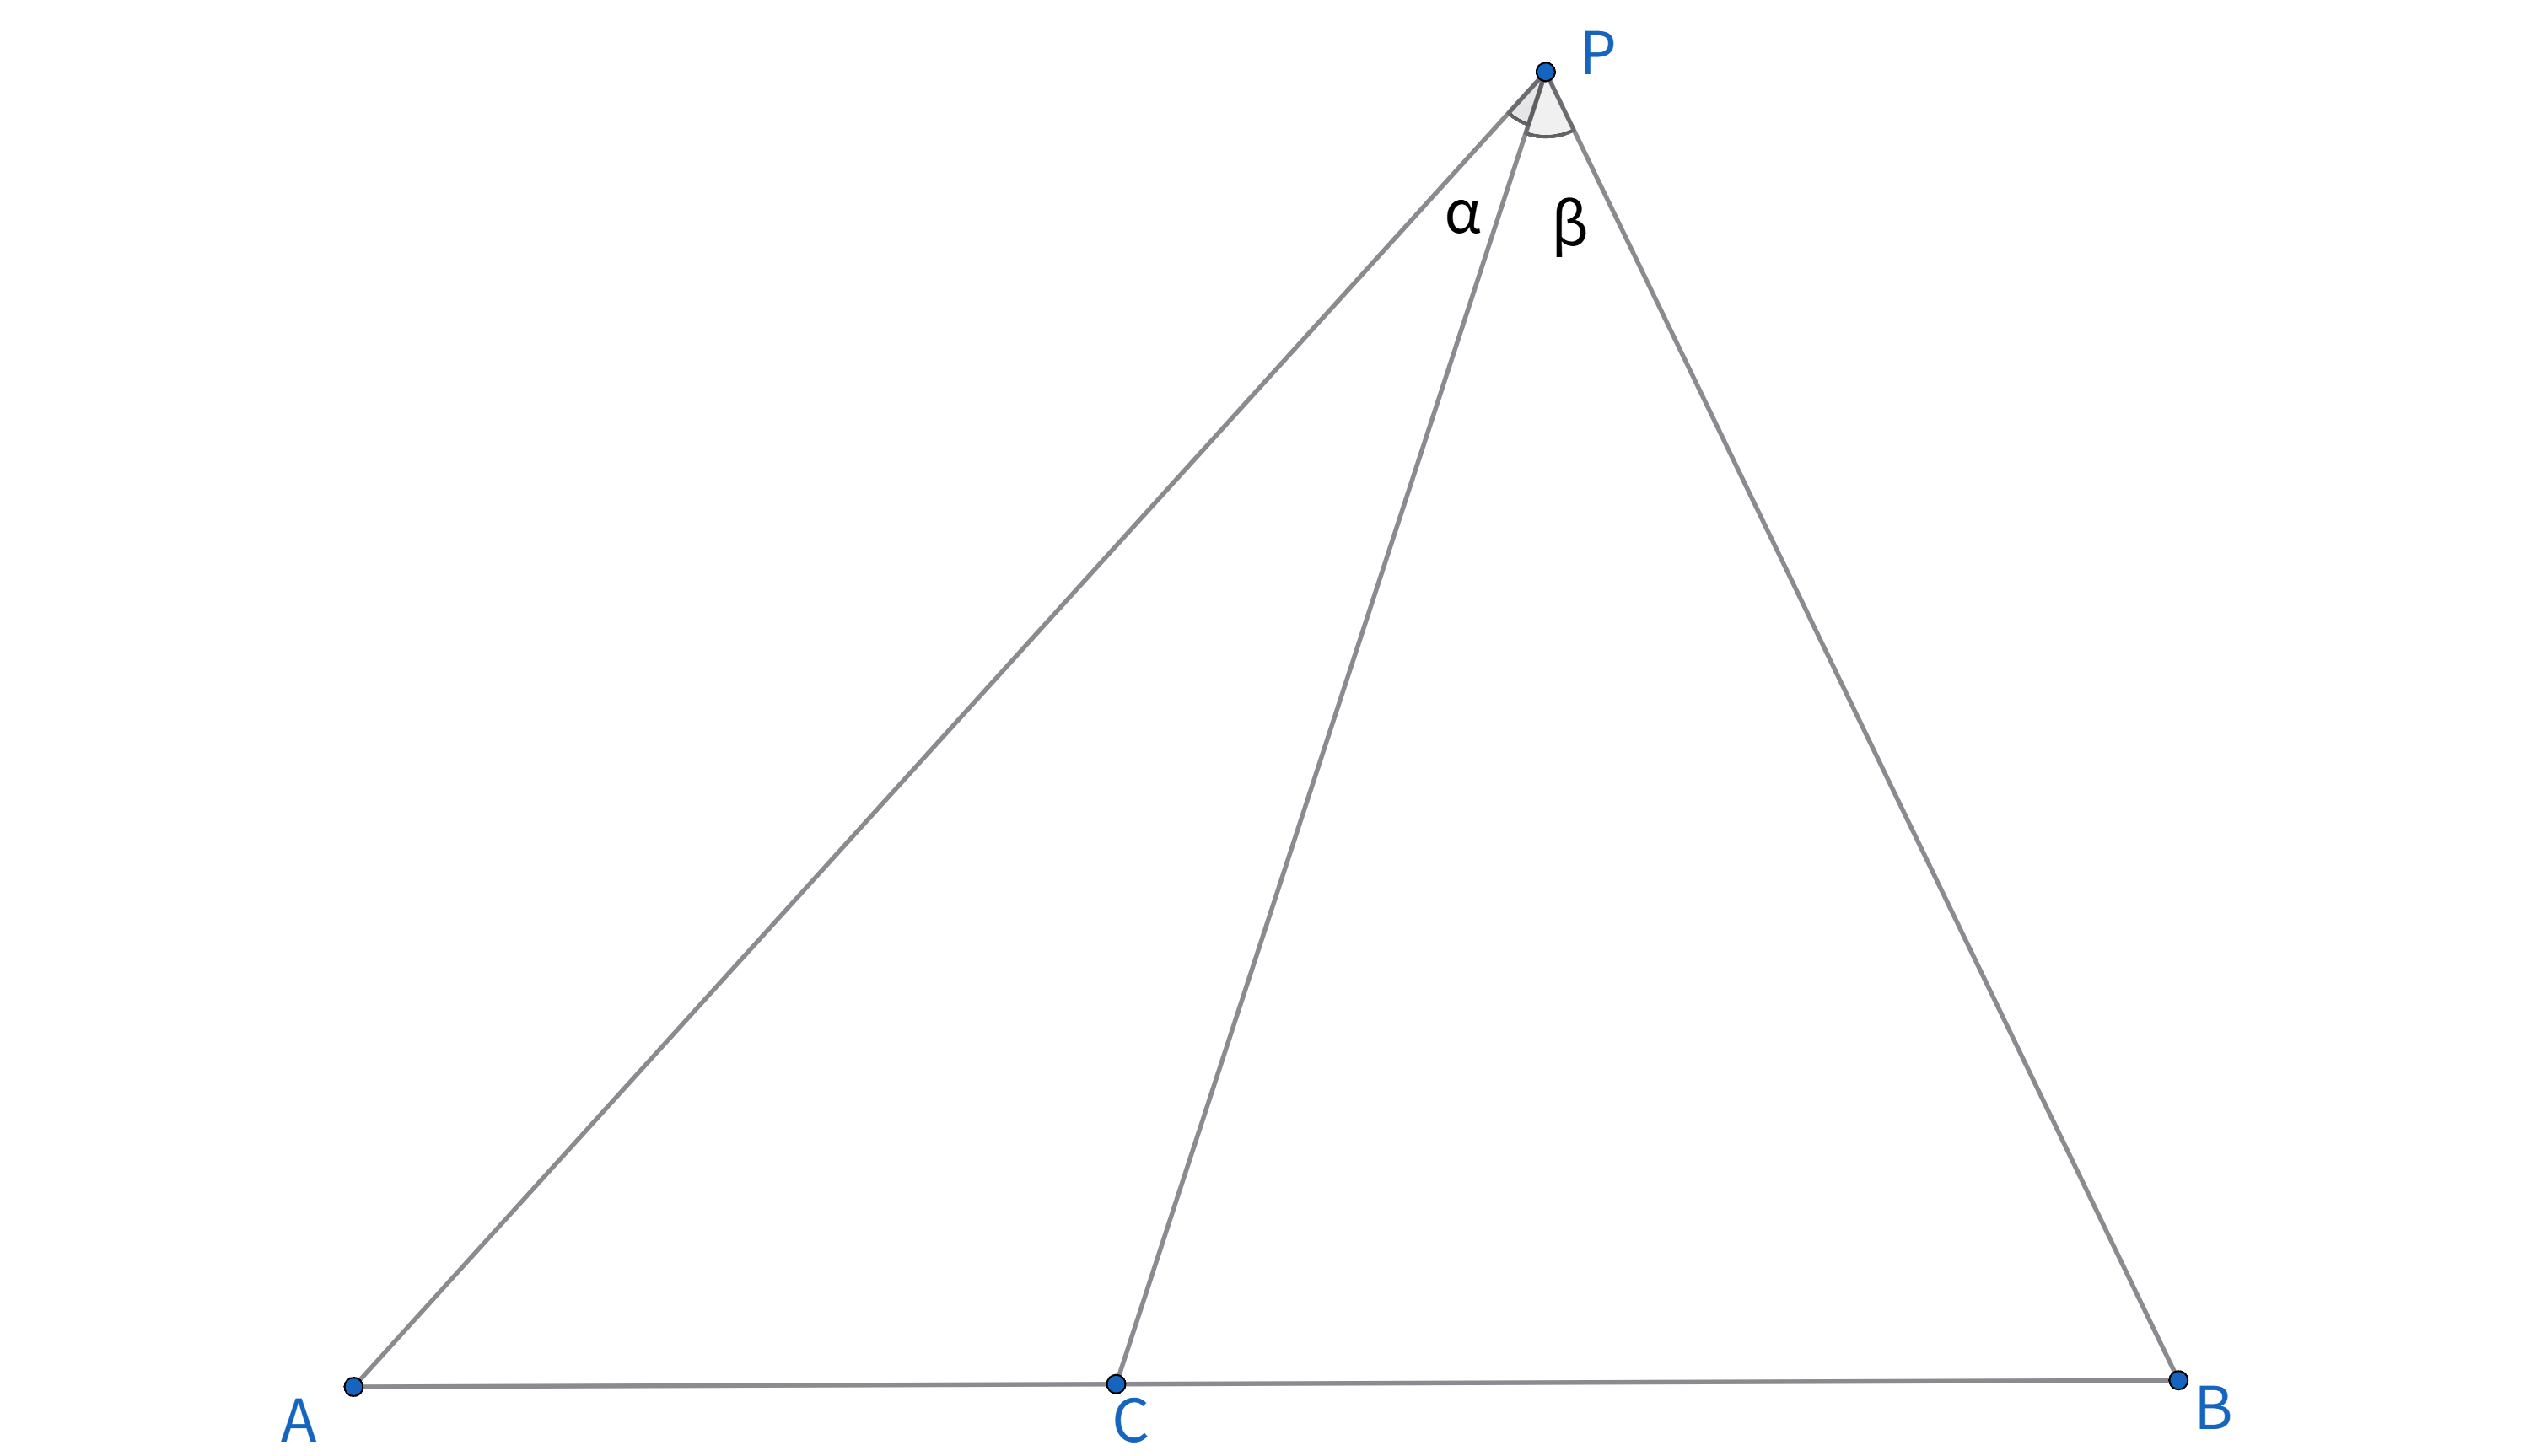
\includegraphics[width=0.7\linewidth]{figures/张角定理.png}
    \caption{张角定理}
\end{figure}


\newpage 
\subsection{定差幂线}
\begin{definition}
    
\end{definition}